\documentclass[10pt,handout]{beamer}
%\documentclass[10pt]{beamer}
\usepackage[english]{babel} % Anpassa efter svenska. Ger svensk logga.
\usepackage[utf8]{inputenc} % Anpassa efter linux
\usepackage{graphicx}
\usepackage{hyperref}
\usepackage{listings}

\hypersetup{
    colorlinks=true,
    linkcolor=blue,
    filecolor=magenta,
    urlcolor=cyan,
}
\usepackage{../common/beamerthemeUppsala}
%\usetheme{Uppsala}
%\usecolortheme{UU} % Anpassa efter UU:s frger och logga
%\hypersetup{pdfpagemode=FullScreen} % Adobe Reader ska ppna fullskrm
\setbeamertemplate{itemize items}[circle]

% \usepackage{beamerthemesplit}
\usepackage{amsmath}
% \usepackage{amssymb}
% \usepackage{graphics}
% \usepackage{graphicx}
% \usepackage{epsfig}
% \usepackage[latin1]{inputenc}
 \usepackage{color}
% \usepackage{fancybox}
% \usepackage{psfrag}
% \usepackage[english]{babel}
 \setbeamertemplate{footline}{\hfill\insertframenumber/\inserttotalframenumber}

% Input new commands
%\usepackage{bm}
%\usepackage{natbib}
\newcommand{\bfm}[1]   {\mbox{\boldmath{${#1}$}}}
\newcommand{\Prob}   {\mbox{\textnormal{P}}}
\def\eqd{\,{\buildrel d \over =}\,}

% Vector/Matrix definitions (in bold type)
\newcommand{\vect}[1]{\mathbf{#1}}
\newcommand{\vectb}[1]{\bm{#1}}

% Differential operator 'd' as upright as in (use \dd)
\newcommand{\dd}{\; \mathrm{d}}

% Gaussian normal distribution (use \N)
\newcommand{\N}{\mathcal{N}} %% or \mathrm{N}

% Uniform distribution (use \Uni or \U)
\newcommand{\Uni}{\mathcal{U}} %% or \mathrm{U}
\newcommand{\U}{\mathcal{U}} %% or \mathrm{U}

% Matrix transpose (use \T)
\newcommand{\T}{^{\mathsf{T}}}

% Blockdiagonal matrices (use \blockdiag)
\newcommand{\blockdiag}{\mathrm{blockdiag}}

% Define inner product '<f,g>' notation (use \innerp{#1})
\providecommand{\innerp}[1]{\left\langle#1\right\rangle}

\def\o{{\mathbf o}}
\def\t{{\mathbf \theta}}
\def\w{{\mathbf w}}
\def\x{{\mathbf x}}
\def\y{{\mathbf y}}
\def\z{{\mathbf z}}



% Other math symbols and notation
\newcommand{\D}{^\mathsf{\dagger}}
\newcommand{\R}{\mathbb{R}}
\newcommand{\erf}{\mathrm{erf}}
\newcommand{\E}{\mathrm{E}}
\newcommand{\var}{\mathrm{var}}
\newcommand{\Var}{\mathrm{Var}}
\newcommand{\cov}{\mathrm{cov}}
\newcommand{\Ker}{\operatorname{Ker}}
\newcommand{\Ran}{\operatorname{Ran}}
\providecommand{\norm}[1]{\lVert#1\rVert}
\providecommand{\op}[1]{\mathcal{#1}}
\newcommand{\arccot}{\mathrm{arccot}}
\providecommand{\Hspace}[1]{\mathscr{#1}}
\providecommand{\fourier}[1]{\mathscr{#1}}

\newcommand{\kin}{k^{\rm in}}
\newcommand{\kout}{k^{\rm out}}
\newcommand{\gi}{{R_0}}
\newcommand{\eff}{{E_{\rm max}}}
\newcommand{\ESS}{\mathrm{ESS}}
\newcommand{\HN}{{\rm N^+}}
\newcommand{\lN}{{\rm LN}}

\DeclareMathOperator{\Sd}{Sd}
\DeclareMathOperator{\sd}{sd}
\DeclareMathOperator{\Gammad}{Gamma}
\DeclareMathOperator{\Invgamma}{Inv-gamma}
\DeclareMathOperator{\Bin}{Bin}
\DeclareMathOperator{\Negbin}{Neg-bin}
\DeclareMathOperator{\Poisson}{Poisson}
\DeclareMathOperator{\Beta}{Beta}
\DeclareMathOperator{\logit}{logit}
\DeclareMathOperator{\BF}{BF}
\DeclareMathOperator{\Invchi2}{Inv-\chi^2}
\DeclareMathOperator{\NInvchi2}{N-Inv-\chi^2}
\DeclareMathOperator{\InvWishart}{Inv-Wishart}
\DeclareMathOperator{\tr}{tr}
% \DeclareMathOperator{\Pr}{Pr}
\def\euro{{\footnotesize \EUR\, }}
\DeclareMathOperator{\rep}{\mathrm{rep}}


%%%%%%%%%%%%%%%%%%%%%%%%%%%%%%%%%%%%%%%%%%%%%%%%%%%%%%%%%%%%%%%%%%

\setlength{\parskip}{3mm}
\title[]{{\color{black}Bayesian Statistics and Data Analysis \\ Lecture 1}}
\author[]{M{\aa}ns Magnusson \\ Department of Statistics, Uppsala University \\ Thanks to Aki Vehtari, Aalto University}
\date{}

\begin{document}

\frame{\titlepage
% \thispagestyle{empty}
}

%%%%%%%%%%%%%%%%%%%%%%%%%%%%%%%%%%%%%%%%%%%%%%%%%%%%%%%%%%%%%%%%%%


\section{Introduction}
\frame{\sectionpage}
\begin{frame}
  \frametitle{Binomial: known $\theta$}

  \begin{itemize}
  \item Probability of event 1 in trial is $\theta$
  \item<2-> Probability of event 2 in trial is $1-\theta$
  \item<3-> Probability of several events in independent trials is e.g.\\
    $\theta\theta(1-\theta)\theta(1-\theta)(1-\theta)\ldots$
  \item<4-> If there are $n$ trials and we don't care about the order
    of the events, then the probability that event 1 happens {\color{red}$y$} times
    is
    \begin{align*}
      p({\color{red}y}|\theta,n) = \binom{n}{{\color{red}y}} \theta^{\color{red}y}(1-\theta)^{n-{\color{red}y}}
    \end{align*}
  \end{itemize}

%   \begin{center}
%   \only<2>{\includegraphics[width=9cm]{dbinom1.pdf}}
%   \only<3>{\includegraphics[width=9cm]{dbinom10.pdf}}
%   \only<4>{\includegraphics[width=9cm]{dbinom10b.pdf}}
% \end{center}
\end{frame}

\begin{frame}
  \frametitle{Binomial: known $\theta$}

  \begin{itemize}
  \item {\color{blue}Observation model} (function of {\color{red} $y$}, discrete)
    \begin{align*}
      p({\color{red}y}|\theta,n) = \binom{n}{{\color{red}y}} \theta^{\color{red}y}(1-\theta)^{n-{\color{red}y}}
    \end{align*}
  \end{itemize}

  \begin{center}
    \only<2>{\includegraphics[width=9cm]{figs/dbinom1.pdf}}
  \end{center}
\end{frame}

\begin{frame}
  \frametitle{Binomial: known $\theta$}

  \begin{itemize}
  \item {\color{blue}Observation model} (function of {\color{red} $y$}, discrete)
    \begin{align*}
      p({\color{red}y}|\theta,n) = \binom{n}{{\color{red}y}} \theta^{\color{red}y}(1-\theta)^{n-{\color{red}y}}
    \end{align*}
  \end{itemize}

  \begin{center}
    {\includegraphics[width=9cm]{figs/dbinom10.pdf}\\
      \vspace{-0.6\baselineskip}
\uncover<2>{\hspace{-18mm}\scriptsize    $p({\color{red}y}|n=10,\theta=0.5)$:\, 0.00 0.01 0.04 0.12 0.21 0.25 0.21 0.12 0.04 0.01 0.00}}
\end{center}
\end{frame}

\begin{frame}
  \frametitle{Binomial: known $\theta$}

  \begin{itemize}
  \item {\color{blue}Observation model} (function of {\color{red} $y$}, discrete)
    \begin{align*}
      p({\color{red}y}|\theta,n) = \binom{n}{{\color{red}y}} \theta^{\color{red}y}(1-\theta)^{n-{\color{red}y}}
    \end{align*}
  \end{itemize}

  \begin{center}
  \only<1>{\includegraphics[width=9cm]{figs/dbinom10b.pdf}\\
      \vspace{-0.6\baselineskip}
{\hspace{-18mm}\scriptsize    $p({\color{red}y}|n=10,\theta=0.9)$:\, 0.00 0.00 0.00 0.00 0.00 0.00 0.01 0.06 0.19 0.39 0.35}}
    \only<2>{\includegraphics[width=9cm]{figs/dbinom10.pdf}\\
      \vspace{-0.6\baselineskip}
{\hspace{-22mm}\scriptsize    $p({\color{red}y}=6|n=10,\theta=0.5)$:\, 0.00 0.01 0.04 0.12 0.21 0.25 \textbf{0.21} 0.12 0.04 0.01 0.00}}
  \only<3>{\includegraphics[width=9cm]{figs/dbinom10b.pdf}\\
      \vspace{-0.6\baselineskip}
{\hspace{-22mm}\scriptsize    $p({\color{red}y}=6|n=10,\theta=0.9)$:\, 0.00 0.00 0.00 0.00 0.00 0.00 \textbf{0.01} 0.06 0.19 0.39 0.35}}
\end{center}
\end{frame}

\begin{frame}
  \frametitle{Binomial: unknown $\theta$}

  \begin{itemize}
  \item Posterior with Bayes rule (function of $\theta$, continuous)
    \begin{equation*}
      p(\theta|y,n,M)=\frac{p(y|\theta,n,M)p(\theta|n,M)}{p(y|n,M)}
    \end{equation*}
    \pause
    where $p(y|n,M)=\int p(y|\theta,n,M)p(\theta|n,M) d\theta$
  \item<3-> Start with uniform prior
    \begin{align*}
      p(\theta|n,M)=p(\theta|M)=1,\, \text{when}\,\, 0\leq\theta\leq 1
    \end{align*}
  \item<4-> Then
    \begin{align*}
      p(\theta|y,n,M)&=\frac{p(y|\theta,n,M)}{p(y|n,M)}
      =\frac{\binom{n}{y} \theta^y(1-\theta)^{n-y}}{\int_0^1
        \binom{n}{y} \theta^y(1-\theta)^{n-y} d\theta} \\
        &=\frac{1}{Z}\theta^y(1-\theta)^{n-y}
    \end{align*}
  \end{itemize}

\end{frame}

\begin{frame}
  \frametitle{Binomial: unknown $\theta$}

  \begin{itemize}
  \item Normalization term $Z$ (constant given $y$)
    \begin{equation*}
      Z= \int_0^1 \theta^y(1-\theta)^{n-y} d\theta = \frac{\Gamma(y+1)\Gamma(n-y+1)}{\Gamma(n+2)}
    \end{equation*}
  \item Normalisation term has \emph{Beta} function form
    \begin{itemize}
    \item when integrated over $(0,1)$
      the result can presented with Gamma functions
    \item with integers  $\Gamma(n)=(n-1)!$
    \item for large integers even this is challenging and usually
      $\log \Gamma(\cdot)$ is computed instead of $\Gamma(\cdot)$
    \end{itemize}
  \end{itemize}

\end{frame}

\begin{frame}
  \frametitle{Binomial: unknown $\theta$}

  \begin{itemize}
  \item Posterior is
    \begin{align*}
      p(\theta|y,n,M) = \frac{\Gamma(n+2)}{\Gamma(y+1)\Gamma(n-y+1)}\theta^y(1-\theta)^{n-y},
    \end{align*}
    \only<2>{
    which is called Beta distribution
    \begin{align*}
      \theta|y,n \sim \text{Beta}(y+1,n-y+1)
    \end{align*}}
  \end{itemize}
  \vspace{0.5\baselineskip}
  \begin{center}
    \only<2>{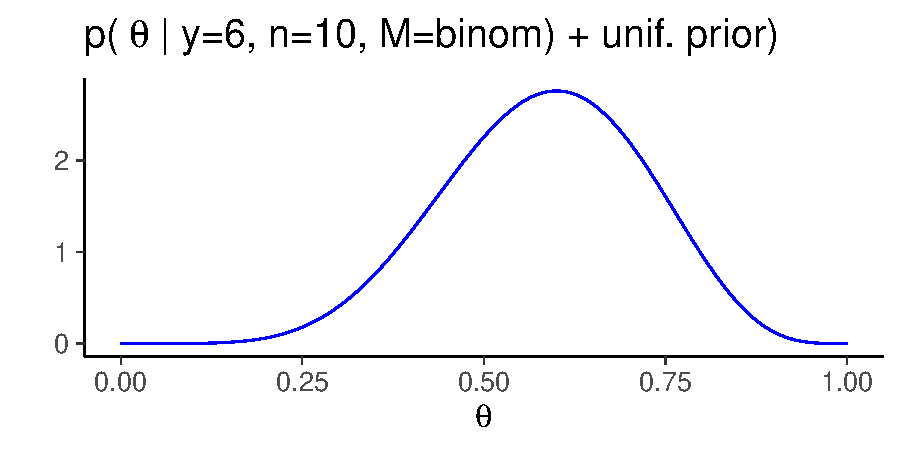
\includegraphics[width=9cm]{figs/dbbeta10c.pdf}}
  \end{center}
\end{frame}

\begin{frame}
  \frametitle{Binomial: computation}

  \begin{itemize}
  \item R
    \begin{itemize}
    \item density {\tt dbeta}
    \item CDF {\tt pbeta}
    \item quantile {\tt qbeta}
    \item random number {\tt rbeta}
    \end{itemize}
  \item Python
    \begin{itemize}
    \item {\tt from scipy.stats import beta}
    \item density {\tt beta.pdf}
    \item CDF {\tt beta.cdf}
    \item prctile {\tt beta.ppf}
    \item random number {\tt beta.rvs}
    \end{itemize}
  \end{itemize}

\end{frame}

\begin{frame}
  \frametitle{Binomial: computation*}

  \begin{itemize}
  \item Beta CDF not trivial to compute
  \item For example, {\tt pbeta} in R uses a continued fraction with
    weighting factors and asymptotic expansion
  \item Laplace developed normal approximation (Laplace
    approximation), because he didn't know how to compute Beta CDF
  \end{itemize}
  % Lagandre, Gamma function

\end{frame}
% Beta distribution named by C. Gini 1911

\begin{frame}
  \frametitle{Placenta previa}

  \begin{itemize}
  \item Probability of a girl birth given placenta previa (BDA3 p. 37)
    \begin{itemize}
    \item 437 girls and 543 boys have been observed
    \item is the ratio 0.445 different from the population average 0.485?
    \end{itemize}
  \end{itemize}
  \pause
  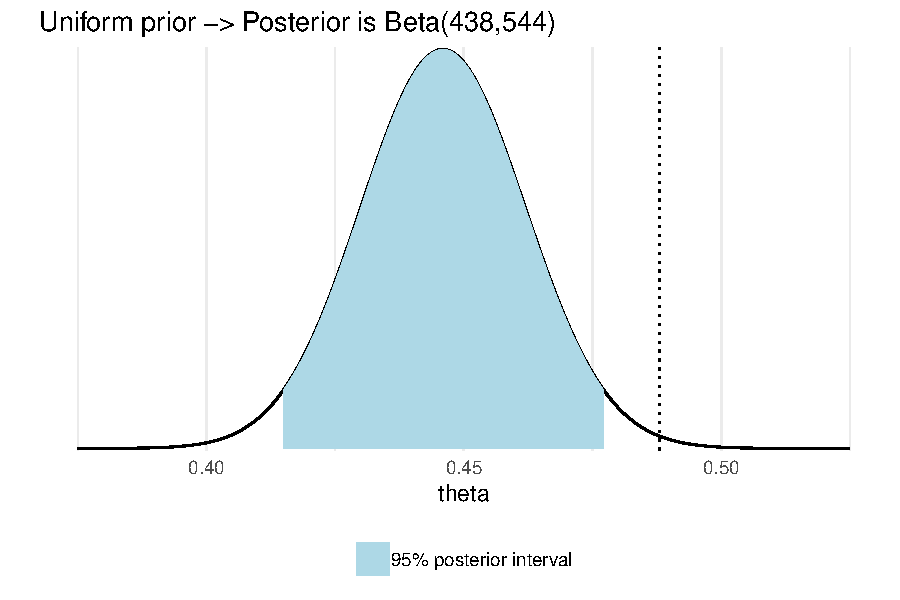
\includegraphics[width=9cm]{figs/demo2_1.pdf}
\end{frame}




%%%%%%%%%%%%%%%%%%%%%%%%%%%%%%%%%%%%%%%%%%%%%%%%%%%%%%%%%%%%%%%%%%


\end{document}
